\section{Dynamic memory allocation}

Memory allocation is mainly a computer hardware operation which is managed through operating system and software applications. Its process is pretty similar to the physical and virtual memory management. Programs and services are assigned with a specific memory as per their requirements when they are executed. Once the program has finished its operation or is idle, the memory is released and allocated to another program or merged within the primary memory.\\

Memory allocation has two core types:
\begin{itemize}
\item Static Memory Allocation: The program is allocated memory at compile time.
\end{itemize}

\begin{itemize}
\item Dynamic Memory Allocation: The programs are allocated with memory at run time.
\end{itemize}

In this report, we will focus on the dynamic allocation of memory and its operation.

\subsection{User interface}

Dynamic Memory Allocation refers to managing system memory is when an executing program requests that the operating system give it a block of main memory. The program then uses this memory for some purpose. Usually the purpose is to add a node to a data structure. In object oriented languages, dynamic memory allocation is used to get the memory for a new object.\\

The memory comes from above the static part of the data segment. Programs may request memory and may also return previously dynamically allocated memory. Memory may be returned whenever it is no longer needed. Memory can be returned in any order without any relation to the order in which it was allocated. The heap may develop ``holes'' where previously allocated memory has been returned between blocks of memory still in use.\\

A new dynamic request for memory might return a range of addresses out of one of the holes. But it might not use up all the hole, so further dynamic requests might be satisfied out of the original hole.\\

If too many small holes develop, memory is wasted because the total memory used by the holes may be large, but the holes cannot be used to satisfy dynamic requests. This situation is called memory fragmentation \cite{Knuth73a}. Keeping track of allocated and deallocated memory is complicated. A modern operating system does all this.\\

Two functions make it possible to reserve and release dynamically an area of memory: \code{malloc()} for the reservation and the liberation of previously allocated memory via \code{malloc()} is provided by the \code{free()} function \cite{WikipediaDMA}.

\subsubsection{Memory allocation}
malloc is a C Standard Library function which is used to allocate a block of memory on the heap. The program accesses this block of memory via a pointer that malloc returns.
The function signature is:

\begin{lstlisting}[style=cstyle]
void* malloc(size_t size);
\end{lstlisting}

The only parameter to pass to malloc is the number of bytes to allocate. The returned value is the address of the first byte of the allocated memory area. If the allocation could not be realized (due to lack of free memory), the return value is the \code{NULL} constant.

\subsubsection{Memory release}
When memory returned by \code{malloc()} is no longer useful, it doesn't get freed on its own. In the order to release the space allocated before we should explicitly use another C Standard Library function: \code{free()} .
The function signature is:
\begin{lstlisting}[style=cstyle]
void free(void *ptr);
\end{lstlisting}
\code{free()} frees the memory space pointed by ptr, which was obtained on a previous call to \code{malloc()}. If it has already been released with \code{free(ptr)}, the behavior is undetermined. If ptr is \code{NULL}, no attempt to release takes place.

\subsection{Goal for good allocators}
An allocator must keep tracking parts of the memory which are in use and free.
The main goals of a good allocator are \cite{Lea12}:
\begin{itemize}
\item Maximizing compatibility
\end{itemize}
The implemented allocator must be compatible with ANSI/POSIX conventions.

\begin{itemize}
\item Maximizing portability
\end{itemize}
The allocator must cover as many systems as possible.
\begin{itemize}
\item Minimizing space
\end{itemize}
The allocator shouldn't waste space and track contiguous chunk to minimize fragmentation.

\begin{itemize}
\item Minimizing time
\end{itemize}
The time for allocation and release of memory should be as short as possible.

\begin{itemize}
\item Maximizing tunability
\end{itemize}
Optional features and behavior should be controllable by users either statically (via \code{#define} and the like) or dynamically (via control commands such as \code{mallopt}).
\begin{itemize}
\item Maximizing Locality
\end{itemize}
Allocating chunks of memory that are typically used together near each other. This helps minimize page and cache misses during program execution.
\begin{itemize}
\item Maximizing error detection
\end{itemize}
It does not seem possible for a general-purpose allocator to also serve as general-purpose memory error testing tool such as Purify. However, allocators should provide some means for detecting corruption due to overwriting memory, multiple frees, and so on.
%\clearpage
\section{Heap and System call}
In the order to implement malloc, we need to understand how memory is handled in most operating systems.We will keep an abstract point of view for that part, since many details are system and
hardware dependent.

\subsection{The Process’s Memory}
Every process has its own virtual address space which is dynamically translated into physical memory  address space by the memory management unit ``MMU'', (and the kernel.) This space is divided in several parts, and what we should know is that we have found at least some space for the code, a stack where local and volatile data are stored, some space for constant and global variables and an unorganized space for program’s data called the heap.\\

The heap is a continuous (in terms of virtual addresses) space of memory blocks with three bounds: a starting point, a maximum limit (managed through \code{sys/resource.h}’s functions \code{getrlimit()} and \code{setrlimit()}) and an end point called the break. The break marks the end of the mapped memory space, that is, the part of the virtual address space that has correspondence into real memory \cite{WilsonJNB95}.\\

\begin{figure}[H]
    \begin{center}
        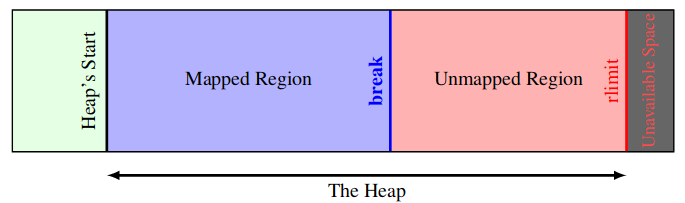
\includegraphics[width=0.8\textwidth]{figures/heap}
    \caption{Memory organisation}
    \label{default}
    \end{center}
\end{figure}

\subsection{Syscalls}
We need to know where the heap begin, the break point position,and of course we need to be able to move the break to implement malloc. This is the purpose of the two syscalls \code{brk()} and \code{sbrk()}.\\

The functions signature are:
\begin{lstlisting}[style=cstyle]
int brk(const void *addr);
void* sbrk(intptr_t incr);
\end{lstlisting}

\code{brk()} and \code{sbrk()} change the location of the program break, which defines the end of the process's data segment (i.e., the program break is the first location after the end of the uninitialized data segment). Increasing the program break has the effect of allocating memory to the process; decreasing the break deallocates memory.

\code{brk()} sets the end of the data segment to the value specified by addr, when that value is reasonable, the system has enough memory, and the process does not exceed its maximum data size.

\code{sbrk()} increments the program's data space by increment bytes. Calling \code{sbrk()} with an increment of 0 can be used to find the current location of the program break.

On success, \code{brk()} returns zero. On error, -1 is returned, and \code{errno} is set to \code{ENOMEM}.

On success, \code{sbrk()} returns the previous program break. (If the break was increased, then this value is a pointer to the start of the newly allocated memory). On error, \code{(void *) -1} is returned, and \code{errno} is set to \code{ENOMEM}.\\

\subsubsection{Example:}

\begin{lstlisting}[style=cstyle]
void minit(int size) 
{ hst=sbrk(size); hli=sbrk(0); }
\end{lstlisting}

\begin{figure}[htbp]
    \begin{center}
        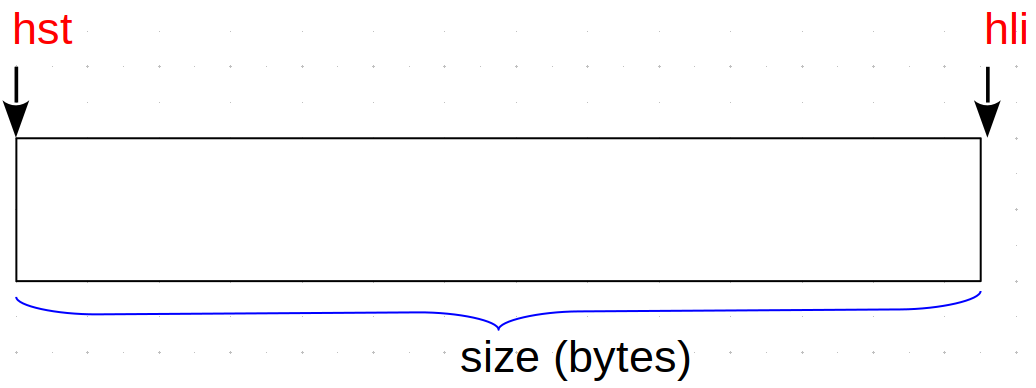
\includegraphics[width=0.8\textwidth]{figures/sbrk}
    \caption{System call for memory extension}
    \label{}
    \end{center}
\end{figure}

We will use \code{sbrk()} as main tool to implement malloc because the only thing we need is to acquire more space (if needed) to fulfill queries.

\section{How to implement allocator}
 Allocators are categorized by the mechanism they use to track which part of the memory is free and coalescing free chunks.
In what follows, I will explain step by step the design of several allocators.

\subsection{How to represent block information}
At the beginning of every chunk,we should have a small block that contains the extra-informations, called meta-data. This block should contain some informations like pointer on the previous and next chunk, a flag to mark free chunks and the data chunk size and it is placed before the pointer returned by malloc.

\begin{figure}[htbp]
    \begin{center}
        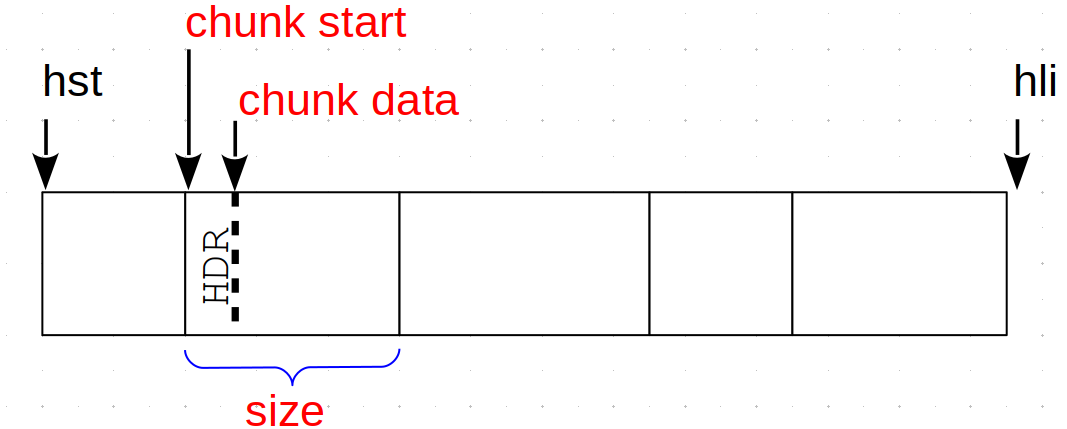
\includegraphics[width=0.8\textwidth]{figures/chunk}
    \caption{Chunk's representation }
    \label{chunkrep}
    \end{center}
\end{figure}

In C we can represent the block by the following structure :
\begin{lstlisting}[style=cstyle]
typedef struct header
{
  size_t size;
  int isfree;
  struct header *prev;
  struct header *nxt;
} header;
\end{lstlisting}

To lighten up our program, we can reduce all this to a simple variable and the meta-data block can be defined in C as:
\begin{lstlisting}[style=cstyle]
typedef size_t header;
\end{lstlisting}

To make the allocation and deallocation operations very simple, another data structure can be used: the free list which operates by connecting unallocated regions of memory together in a linked list \ref{freelist}. In the above structure we the field ``nxt'' will help us to build it.
To implement an allocator with a free list, we can use the structure below:
\begin{lstlisting}[style=cstyle]
typedef struct header
{
  size_t size;			
  struct header *nxt;
} header;
\end{lstlisting}

\begin{figure}[htbp]
    \begin{center}
        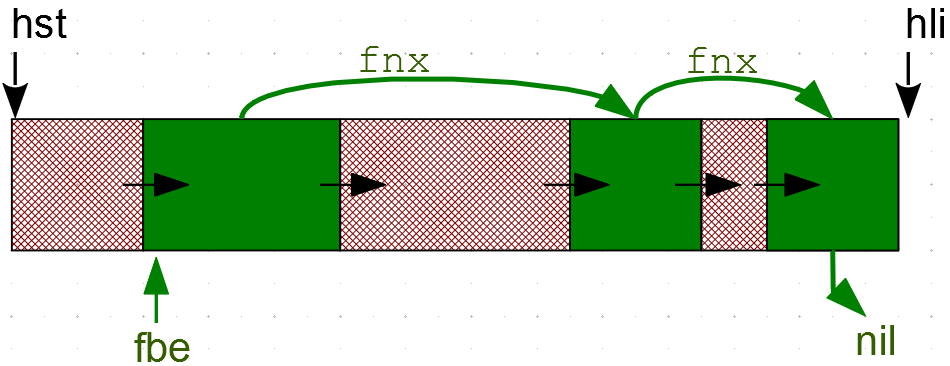
\includegraphics[width=0.8\textwidth]{figures/freelist}
    \caption{Heap with free list in green}
    \label{freelist}
    \end{center}
\end{figure}

Notice that this is quite enough to implement an allocator since we can get the bock size by doing a bitwise operation and the following chunk by summing the current chunk and the size but also encode the free flag in 1 bit with this variable.

\begin{lstlisting}[style=cstyle]
// methods to get header information
#define HDR_GET_SIZE(p)   (p->size & (~1))
#define HDR_GET_STATUS(p)   (p->size & 1)
#define HDR_GET_NEXT(p)   ((header*) p + HDR_GET_SIZE(p))
#define HDR_SET_SIZE(p,nh)  p->size = (((nh + 1) >> 1) << 1) & (~HDR_GET_STATUS(p))
#define HDR_SET_STATUS(p)   p->size = p->size | 1
#define HDR_UNSET_STATUS(p) p->size = p->size & (~1)
\end{lstlisting}

The figure \ref{chunkrep} presents an example of heap organization with meta-data in front of the allocated block. Each data chunk has a meta-data block followed by a data block. Note that the pointer returned by malloc points on the data block, not on the whole chunk.\\

\subsection{Allocation Algorithms}
  One of the important part of malloc is the way that thunk are found and allocated. In what follows, we will discuss some policies and algorithms used to perform a dynamic allocation
%First-fit method
\subsubsection{First-fit method}
The first fit method allocates the process to a partition which is the first sufficient chunk from the top of Main Memory \ref{ff_alg}.

In lazy allocators, if the search fails, a garbage collection will be done, and then try to allocate again.

If there’s still no free block big enough for the process, the only choice is to increase the size of the heap (if possible) with \code{sbrk()}, and then try the allocation again.
If you can’t increase the size of the heap

\begin{figure}[htbp]
    \begin{center}
        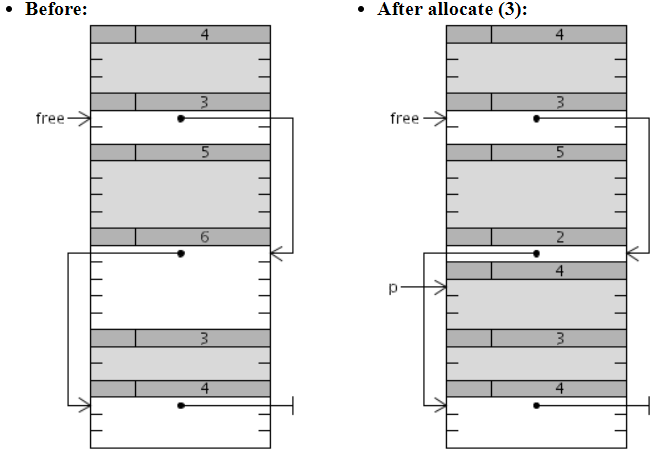
\includegraphics[width=0.8\textwidth]{figures/FF_alg}
    \caption{First fit execution }
    \label{ff_alg}
    \end{center}
\end{figure}

%first fit algorithm
\begin{algorithm}
\caption{Algorithm for allocate (n)}
\begin{algorithmic} 
\REQUIRE $n \geq 0$
\STATE $size(block) \leftarrow n + size(header)$  
\STATE Scan free list for first block with $nWords \geq size(block)$ 
\IF{block not found} 
  \STATE Failure (time for garbage collection!) 
\ELSIF{free block $nWords \geq size(block) + size(header) + 1$} 
   \STATE Split into a free block and an in-use block 
   \STATE Free block $nWords \leftarrow Free block nWords - size(block) $
   \STATE In-use block $nWords \leftarrow size(block) $
    \STATE Return pointer to in-use block 
\ELSE 
    \STATE Unlink block from free list 
    \STATE Return pointer to block 
\ENDIF
\end{algorithmic}
\end{algorithm}

\begin{itemize}
\item Its main advantage is that it is the fastest search as it searches only the first block i.e. enough to assign a process.
\end{itemize}

%best fit algo
\subsubsection{Best-fit method}
The best fit method allocates the process to a partition which is the smallest sufficient partition among the free available partitions in the main memory\ref{bf_alg}.

if the search fails we'll use the same process we describe before in first fit method.

\begin{figure}[htbp]
    \begin{center}
        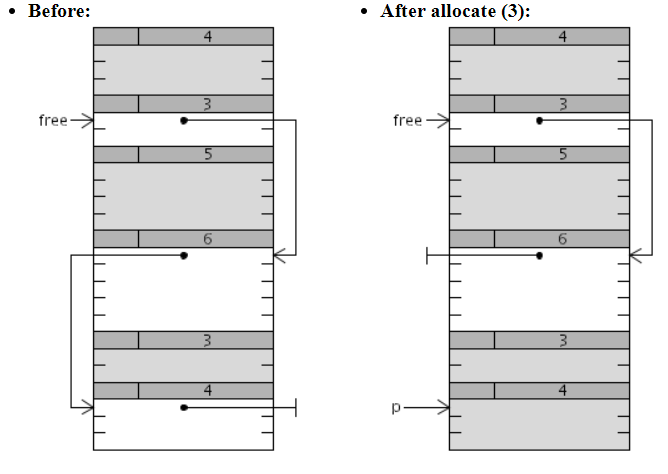
\includegraphics[width=0.8\textwidth]{figures/BF_alg}
    \caption{Best fit execution }
    \label{bf_alg}
    \end{center}
\end{figure}
%best fit algorithm
\begin{algorithm}
\caption{Algorithm for allocate (n)}
\begin{algorithmic} 
\REQUIRE $n \geq 0$

\STATE $size(block) \leftarrow n + size(header)$ 
\STATE Scan free list for smallest block with $ nWords \geq size(block)$ 
\IF{block not found} 
  \STATE  Failure (time for garbage collection!) 
\ELSIF{ $nWords \geq size(block) + size(header) + 1$}
   \STATE Split into a free block and an in-use block 
   \STATE Free block  $nWords = Free block nWords - size(block) $
   \STATE In-use block $nWords = size(block) $
   \STATE Return pointer to in-use block 
\ELSE 
   \STATE Unlink block from free list 
   \STATE Return pointer to block 
\ENDIF

\end{algorithmic}
\end{algorithm}


Although, best fit minimizes the wastage space, it consumes a lot of processor time for searching the block which is close to required size. Also, Best-fit may perform poorer than other algorithms in some cases.
 
